 \chapter{Methodik}
\label{chap:Methodik}

% Ziel hier: den Leser in die Lage versetzen, die wesentliche Struktur der Arbeit nachvollziehen zu können (Vorgehen / Geräte / Materialien / Verfahren [also auch Software]  / getroffene Annahmen ... sollten hier erklärt werden)

\section{PCM}
\label{sec:pcm}
Hier Steht was zu \ac{pcm}
\begin{figure}[H]
    \centering

    \begin{subfigure}{0.9\textwidth}
        \centering
        \includegraphics[width=\linewidth]{../../Code/pcm_mass.pdf}
        \caption{PCM Masse}
        \label{fig:pcm_mass}
    \end{subfigure}

    \vspace{1em}  % Optional vertical spacing

    \begin{subfigure}{0.9\textwidth}
        \centering
        \includegraphics[width=\linewidth]{../../Code/pcm_heat_capacity.pdf}
        \caption{PCM Wärmeaufnahme}
        \label{fig:pcm_heat}
    \end{subfigure}

    \caption{PCM Auslegung}
    \label{fig:pcm_mass_heat}
\end{figure}

\newpage

\section{Radiator}
\label{sec:Radiator}
Hier steht was zu Radiatoren.

\begin{figure}[H]
  \centering
  \includegraphics[width=\linewidth]{../../Code/radiator_leistung.pdf}
  \caption{Radiator Leistung nach Fläche und Temperatur}
  \label{fig:pcm_heatflux}
\end{figure}

\newpage

\section{PCM Radiator Hybrid}
\label{sec:pcmRadiatorHybrid}
Eine Hybridlösung wird auch in erwägung gezogen, um die Masse durch nutzung eines Radiators zu minimieren, wobei wegen aerodynamischer Aufheizung für kurze Zeit ein PCM gebraucht werden könnte.
Um eine umständliche Simulation mittels \ac{cfd} zu vermeiden, wird die Außenkontour der Rakete von Spitze bis Avionik-Sektion, mit Hilfe der Nußelt-Beziehungen, als längsangeströmte ebene Platte angesehen,
wie in Abbildung \ref{fig:rakete_kontour} dargestellt ist.
Um zu wissen, ob hier die Beziehung für laminare oder turbulente Grenzschichten angewandt werden soll, müssen zunächst die Gültigkeitsbereiche der Reynolds- und Prandtlzahl (\ref{eq:prandtl}, \ref{eq:reynolds}) überprüft werden.
\begin{equation}
  \label{eq:qdot}
  \dot{q} = \alpha \ (T_r - T_w)
\end{equation}
\begin{equation}
  \label{eq:nusselt_turbulent}
  \text{Nu}_x = \frac{\alpha_x x}{\lambda} = 0,0296 \ \text{Re}_x^{0,8} \ \text{Pr}^{\frac{1}{3}}
\end{equation}
Es gilt folgender Gültigkeitsbereich: $5 \cdot 10^5 \leq \text{Re}_L \leq 10^7$, $0,6 \leq \text{Pr} \leq 60$ und muss berücksichtigt werden,
wobei die Reynoldszahl direkt aus der Trajektorien-Simulation ausgegeben wird, aber zur überprüfung trotzdem auch ausgerechnet wird.
\newline
\noindent\begin{minipage}{.5\linewidth}
\begin{equation}
  \label{eq:reynolds}
  \text{Re}_x = \frac{V \rho x}{\eta}
\end{equation}
\end{minipage}%
\begin{minipage}{.5\linewidth}
\begin{equation}
  \label{eq:prandtl}
  \text{Pr} = \frac{c_p \eta}{\lambda}
\end{equation}
\end{minipage}
Die Dynamische Viskosität wird mittels der Sutherlands-Formel berechnet, und die Recoverytemperatur mittels der adiabaten Strömungsgleichung, welche auch vom Recovery-Faktor abhängt.
\begin{equation}
  \label{eq:dynamische_viskositaet}
  \eta = \eta_0 \frac{T_0 + C}{T_{\infty} + C} \left( \frac{T_{\infty}}{T_0} \right)^{\frac{2}{3}}
\end{equation}
\begin{equation}
  \label{eq:recovery_temperatur}
  T_r = T_{\infty} \left( 1 + r \frac{\kappa + 1}{2} \text{Ma}^2 \right)
\end{equation}
Für turbulente Grenzschichten lässt sich folgende Approximation des Recovery-Faktors anwenden.
\begin{equation}
  \label{eq:recovery_faktor}
  r = \frac{2}{\left(\kappa - 1\right) \text{Ma}_e^2} \left(\frac{T_{a_{w}}}{T_e} - 1\right) \approx \sqrt[3]{\text{Pr}}
\end{equation}

\newpage

% Hybrid PCM ohne aufheizung
\begin{figure}
  \centering
  \begin{tikzpicture}[rotate border/.style={shape border uses incircle, shape border rotate=#1}, scale=0.8]
    \draw[thick] (3,3) -- (3,-1) -- (9,-1) -- (9,3);
    \draw[thick] (3,3) -- node [midway, above] {Avionik Sektion}  (9,3);
    \draw[thick] (4,3) -- (4,-1); % PCM Lamellen
    \draw[thick] (3,-0.5) -- (4,-0.5);
    \draw[thick] (3,0) -- (4,0);
    \draw[thick] (3,0.5) -- (4,0.5);
    \draw[thick] (3,1) -- (4,1);
    \draw[thick] (3,1.5) -- (4,1.5);
    \draw[thick] (3,2) -- (4,2);
    \draw[thick] (3,2.5) -- (4,2.5);
    \node at (-0.5,2) [style={single arrow, draw}, minimum height=3cm, minimum width=0.5cm, thick]{$\dot{Q}_{\mathrm{Umwelt}}$}; % Wärmestrom pfeil
    \node at (-0.5,0) [style={single arrow, draw}, minimum height=4.5cm, minimum width=1.5cm, shape border rotate=180, thick]{$\dot{Q}_{\mathrm{Radiator}}$}; % Wärmestrom pfeil
    \node at (6.5,1)[style={single arrow, draw}, minimum height=3cm, minimum width=0.5cm, shape border rotate=180, thick]{$\dot{Q}_{\mathrm{Avionik}}$}; % Wärmestrom pfeil
    \draw[->, thick, -{Stealth[length=0.25cm]}] (1,3.75) node [above=1pt] {PCM mit Lamellen} -- (3.5,2.6);
  \end{tikzpicture}
  \caption{PCM Wärmestrom ohne aerodynamische Aufheizung}
  \label{fig:pcm_waermestrom_diagramm}
\end{figure}


$\dot{Q}_{\mathrm{Radiator}} = \dot{Q}_{\mathrm{Umwelt}} + \dot{Q}_{\mathrm{Avionik}}$ In diesem Fall reicht die Leistung des Radiators, um die Avionik auf Betriebstemperatur zu halten.

% Hybrid PCM Wärmestrom bei aufheizung
\begin{figure}[H]
  \centering
  \begin{tikzpicture}[rotate border/.style={shape border uses incircle, shape border rotate=#1}, scale=0.8]
    \draw[thick] (3,3) -- (3,-1) -- (9,-1) -- (9,3);
    \draw[thick] (3,3) -- node [midway, above] {Avionik Sektion}  (9,3);
    \draw[thick] (4,3) -- (4,-1); % PCM lamellen
    \draw[thick] (3,-0.5) -- (4,-0.5);
    \draw[thick] (3,0) -- (4,0);
    \draw[thick] (3,0.5) -- (4,0.5);
    \draw[thick] (3,1) -- (4,1);
    \draw[thick] (3,1.5) -- (4,1.5);
    \draw[thick] (3,2) -- (4,2);
    \draw[thick] (3,2.5) -- (4,2.5);
    \node at (-0.5,2) [style={single arrow, draw}, minimum height=4.5cm, minimum width=1.5cm, thick]{$\dot{Q}_{\mathrm{Umgebung}}$}; % Wärmestrom pfeil
    \node at (-0.5,0) [style={single arrow, draw}, minimum height=4.5cm, minimum width=1.5cm, shape border rotate=180, thick]{$\dot{Q}_{\mathrm{Radiator}}$}; % Wärmestrom pfeil
    \node at (6.5,1)[style={single arrow, draw}, minimum height=3cm, minimum width=0.5cm, shape border rotate=180, thick]{$\dot{Q}_{\mathrm{Avionik}}$}; % Wärmestrom pfeil
  \end{tikzpicture}
  \caption{PCM Wärmestrom bei aerodynamischer Aufheizung}
  \label{fig:pcm_waermestrom_aufheizung_diagramm}
\end{figure}


Hier reicht die Leistung des Radiators nicht mehr aus, resultierend steigt die Temperatur leicht an (Tut sie nicht, wir nehmen wegen dem PCM die Hauttemperatur als isotherm an,
lediglich gibt es einen infinitesimalen Schritt über den Schmelzpunkt hinweg) und das PCM fängt an zu schmilzen. Zu beachten ist,
dass die Leistung des Radiators durch die Temperaturerhöhung auch steigt.

% Raketenkontour im Luftstrom für ebene Platte Annahme
\begin{figure}[H]
  \centering
  \begin{tikzpicture}
    \draw[thick] (0,0) arc [start angle=90, end angle=270, x radius=5cm, y radius= 1.5cm]; %nosecone
    \draw[thick] (0,0) -- (3,0); % hülle
    \draw[thick] (0,-3) -- (3,-3); % hülle
    \draw[thick] (-5.75,-1.5) -- (-5.25,-1.5); % maß links
    \draw[thick] (1,0.25) -- (1,0.75); % maß rechts
    \draw[thick] (0,0.5) arc [start angle=90, end angle=180, x radius=5.5cm, y radius= 2cm]; % maß bogen
    \draw[thick] (0,0.5) -- node [near start, above] {Länge} (1,0.5); % maß grade sektion
    \draw[->, thick, -{Stealth[length=0.25cm]}] (-10,0.5) -- node [midway, above] {Luftstrom} (-7,0.5); % free stream pfeile
    \draw[->, thick, -{Stealth[length=0.25cm]}] (-10,-0.5) -- (-7,-0.5); % Strompfeile
    \draw[->, thick, -{Stealth[length=0.25cm]}] (-10,-1.5) -- (-7,-1.5);
    \draw[->, thick, -{Stealth[length=0.25cm]}] (-10,-2.5) -- (-7,-2.5);
    \draw[->, thick, -{Stealth[length=0.25cm]}] (-10,-3.5) -- (-7,-3.5);
    \draw[thick] (0,0) -- (0,-2.5); % casing wall
    \draw[thick] (2,0) -- (2,-2.5); % casing wall
    \draw[thick] (0,-2.5) -- (2,-2.5); % casing bottom
    \node at (1,-1.5) [style={single arrow, draw}, minimum height=0.5cm, minimum width=1.5cm, rotate=90, thick]{$\dot{Q}_{\mathrm{Avionik}}$}; % Wärmestrom pfeil
  \end{tikzpicture}
  \caption{Kontourlänge vom Staupunkt der Rakete bis zum Mittelpunkt des Radiators}
  \label{fig:rakete_kontour_zeichnung}
\end{figure}
\newpage
\begin{figure}[H]
  \centering
  \label{fig:pcm_waermestrom_flugsimulation}
  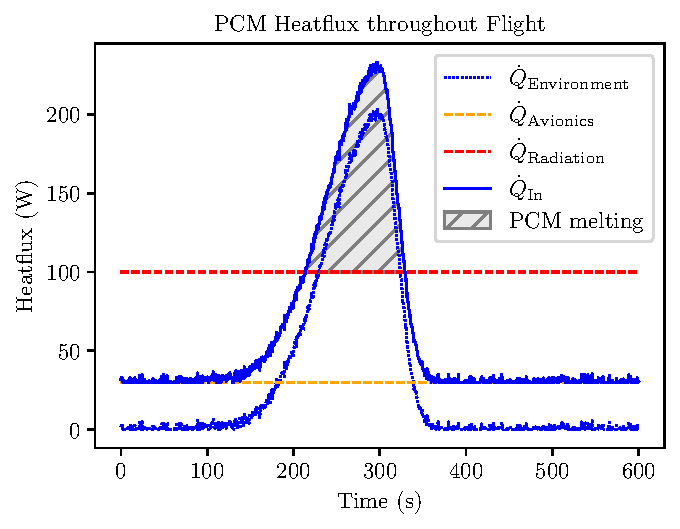
\includegraphics[width=\linewidth]{../../Code/pcm_radiator_hybrid_heatflux_during_flight.pdf}
  \caption{PCM Wärmestrom während Flug}
  \label{fig:re_pr_flugsimulation}
  \includegraphics[width=\linewidth]{../../Code/re_pr_during_flight.pdf}
  \caption{Reynolds- und Prandtlzahl während kritischer Phase im Flug}
\end{figure}

\newpage
Hier sieht man wie die Dimensionierung in den Programmen abläuft. Die Programme erzeugen alle Graphen und rechnen simultan für gegebenen Avionik Wärmestrom alle Werte aus.

\begin{center}
\begin{tikzpicture}[
  sibling distance=10em,
  every node/.style = {
    shape=rectangle,
    rounded corners,
    draw,
    align=center,
    minimum width=3cm
  },
  edge from parent/.style = {
    draw,
    ->,
    -{Stealth[length=0.25cm]},
    thick
  }
]
  % Top tree without PCM Höhe
  \node (avionik) {Avionik Wärmestrom}
    child { node (radiator) {Radiator Fläche}
      child { node (breite) {PCM Breite} }
      child { node (umwelt) {Umwelt Wärmestrom} 
        child { node (kapazitaet) {PCM Kapazität} }
      }
    };

  % Place PCM Höhe manually below and centered between Breite and Kapazität
  \node (hoehe) [below=10em of $(radiator)$] {PCM Höhe}
  	child {node (gewicht) {PCM Gewicht}};

  % Draw straight arrows from both parents to PCM Höhe
  \draw[->, thick, -{Stealth[length=0.25cm]}] (breite) -- (hoehe);
  \draw[->, thick, -{Stealth[length=0.25cm]}] (kapazitaet) -- (hoehe);
\end{tikzpicture}
\end{center}